System Architect - Justin
\section{Block Diagram}
\begin{figure}[H]
\centering
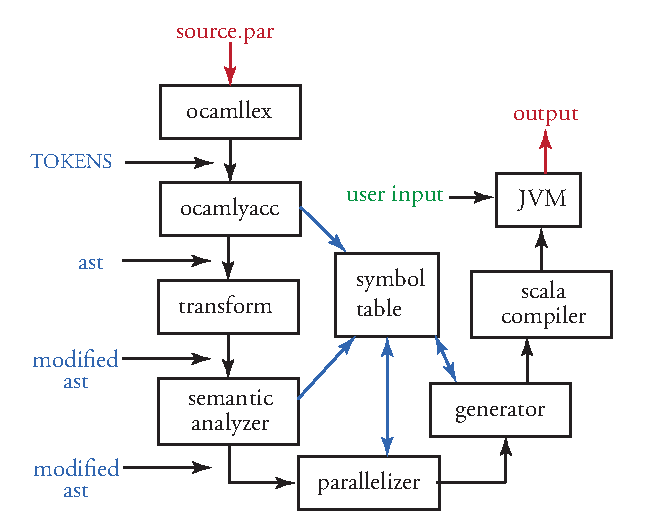
\includegraphics[scale=1]{blockdiagram.eps} 
\caption{Block Diagram of the DotPar compiler.}
\end{figure}

\section{Interfaces}
Dotpars interface, as seen above, follows a standard compiler form. The raw
source file is fed into the \verb=lexer=, \verb=ocamllex=, which outputs a series of tokens that is then
parsed by \verb=ocamlyacc=.  \verb=Ocamlyacc= uses a our custom type system to output an abstract
syntax tree.

Our abstract syntax tree then undergoes a series of modifications and optimizations before it
is complied down into scala and fed into the scala compiler.  The first transform
is done by the aptly named \verb=transform.ml= which reverses nodes with a tree.  The lexer
recurses right to left, and thus all lists are stored backeds and need to be reversed.
The transform outputs a modified AST which is then fed into the semantic analyzer.

The semantic analyzer performs an extensive amount of type checking, making 
sense of a user's source code, throwing errors where appropriate, recovering from 
small errors if possible,  and adding necessary information to the symbol table.  

<<<<<<< HEAD
Next, the parallelizer, in which the main optimizations are performed, takes
the modified AST from the semantic analyzer. The first pass
performs a series of tests to find, and declare certain functions as
\emph{pure}. A second pass marks certain functions as \emph{associative}.
These functions that are pure can be parallelized in maps and list
comprehensions, and pure and associative functions can be parallelized in
reduces as well. Our optimizatinos focus on major bottlenecks of source programs
including maps, reduces, and list comprehensions.

Lastly, the parallelizer outputs a modified AST which is fed into the generator, 
which does a pass over the ast, translating the tree into and creating parallelized 
functions where applicable, which is lastly fed into the scala compiler.  The
scala compiler then complies down the JVM which can then be run on a target machine.
=======
Next is the parallelizer where the main optimizations are acomplished. It takes 
the modified ast from the semantic analyzer and performs two passes to test. 
Each pass performs a series of tests to find, and declare certain functions as \emph{pure}.
These \emph{pure} functions can be parallelized. Our optimizations focus on major
bottlenecks of source programs including maps, reduces, and list comprehensions.

Lastly, the parallelizer outputs a modified ast that is fed into the generator, 
which does a pass over the ast, translating the tree and creating parallelized 
functions where applicable. Finally this is fed into the scala compiler.  The
scala compiler then complies down the JVM, which can then be run on a target machine.
>>>>>>> Updates

Dotpar uses a total of 5 different passes over the abstract syntax, performing 
checks and optimizations at each state to insure relability.  With this comes
the added benefit thgat a program is not required to be parallizable in order to run.  Dotpar
will only attempt to parallelize a program after extensive checks which gives add 
compile security and relability.

\section{Implementation}
<<<<<<< HEAD
The original grammar, written using \verb=yacc= and \verb=lex=, was designed and
implemented Sid Nair and Nathan Hwang. The conversion to OCaml was done by Sid
Nair and Justin Hines. The parsing to create the AST was was completed by
Nathan Hwang and Justin Hines. An additional transformation pass on the tree was
done by Nathan Hwang. The semantic analysis pass was implemented by Justin
Hines and Andrew Hitti. The parallelizer was implemented by Sid Nair with minor
contributions from Justin Hines and Nathan Hwang. The Generator was implemented
by Nathan Hwang with signifcant contributions from Sid Nair, Andrew Hitti, and
Justin Hines. Test cases were written by all group members, but the primary
contributors were Nathan Hwang, Andrew Hitti, and Logan Donovan.
=======
The grammar was designed and implemented Sid Nair, and Nathan Hwang, with the
conversion to Ocaml being carried out by Sid Nair and Justin Hines.  The parser was
completed by Nathan Hwang and Justin Hines.  The transform by Nathan Hwang.  The
Semantic Analyzer was implemented by Justin Hines and Andrew Hitti with help from Logan Donovan.  The Parallelizer was
implemented by Sid Nair with minor contributions by Justin Hines, and Nathan Hwang. 
The Geneator was implemented by Nathan Hwang with signifcant contributions from 
Sid Nair, Andrew Hitti, and Justin Hines.
>>>>>>> Updates
